\documentclass[11pt]{beamer}
\usetheme{Antibes}
\usepackage[utf8]{inputenc}
\usepackage[german]{babel}
\usepackage[T1]{fontenc}
\usepackage{amsmath}
\usepackage{amsfonts}
\usepackage{amssymb}
\usepackage{graphicx}
\author{Gruppe C14 \\ Julián Häck, Martin Koytek, Lars Wenning, Erik Zimmermann}
\usepackage{float}
\usepackage{subfigure}
%\title{}
%\setbeamercovered{transparent} 
%\setbeamertemplate{navigation symbols}{} 
%\logo{} 
%\institute{} 
%\date{} 
%\subject{} 
\begin{document}


%\begin{frame}
%\tableofcontents
%\end{frame}
\section{Rauschmessung}
\subsection{Temperatursensoren}
\begin{frame}
\begin{figure}[H]
    \subfigure[Gruppe 1]{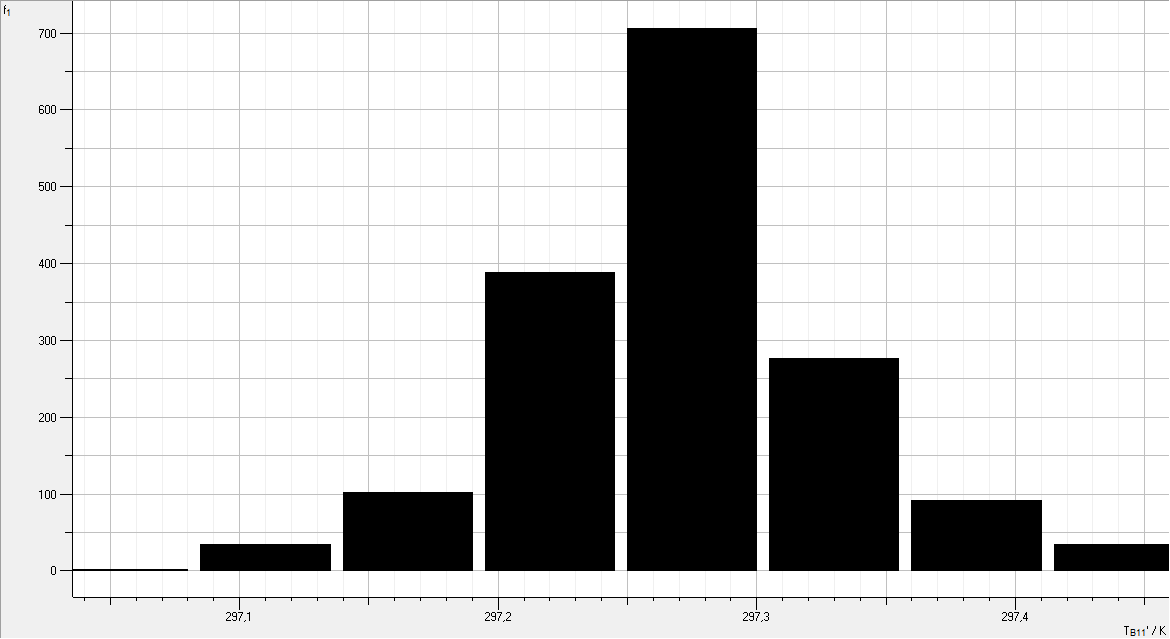
\includegraphics[width=0.49\textwidth]{Bilder/Zimmertemperatur_G1_1.png}}
    \subfigure[Gruppe 2]{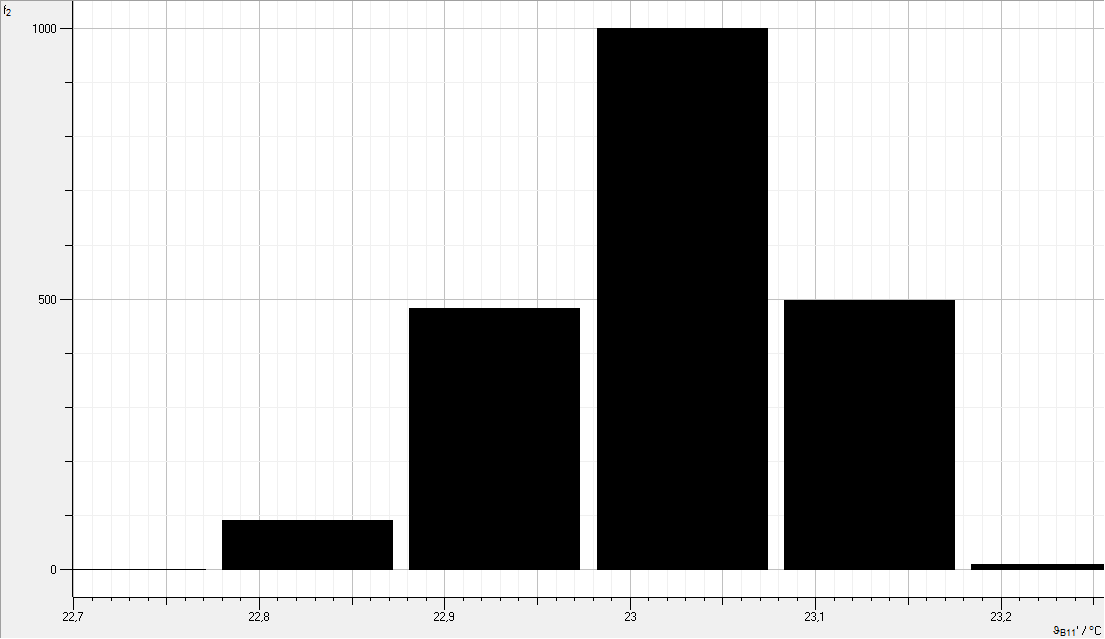
\includegraphics[width=0.49\textwidth]{Bilder/Zimmertemperatur_G2.png}}
\end{figure}
\begin{table}[H]\centering
\begin{tabular}{c|c|c}
 & Gruppe 1 & Gruppe 2 \\ 
\hline 
$T_M$ in K & 297.26 & 296.17 \\ 
$\sigma_T$ in K & 0.054 & 0.069 \\  
\end{tabular} 
\end{table}
\end{frame}



\subsection{Drucksensoren}
\begin{frame}
\begin{figure}[H]
    \subfigure[Gruppe 1]{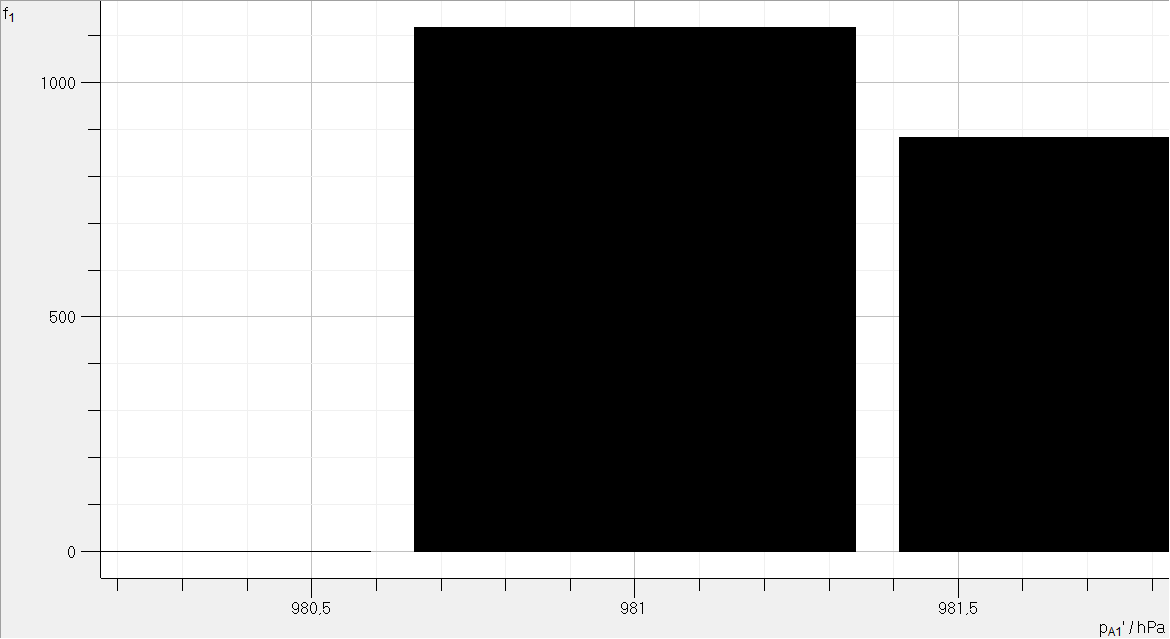
\includegraphics[width=0.49\textwidth]{Bilder/Zimmertemperatur_Druck_G1_1.png}}
    \subfigure[Gruppe 2]{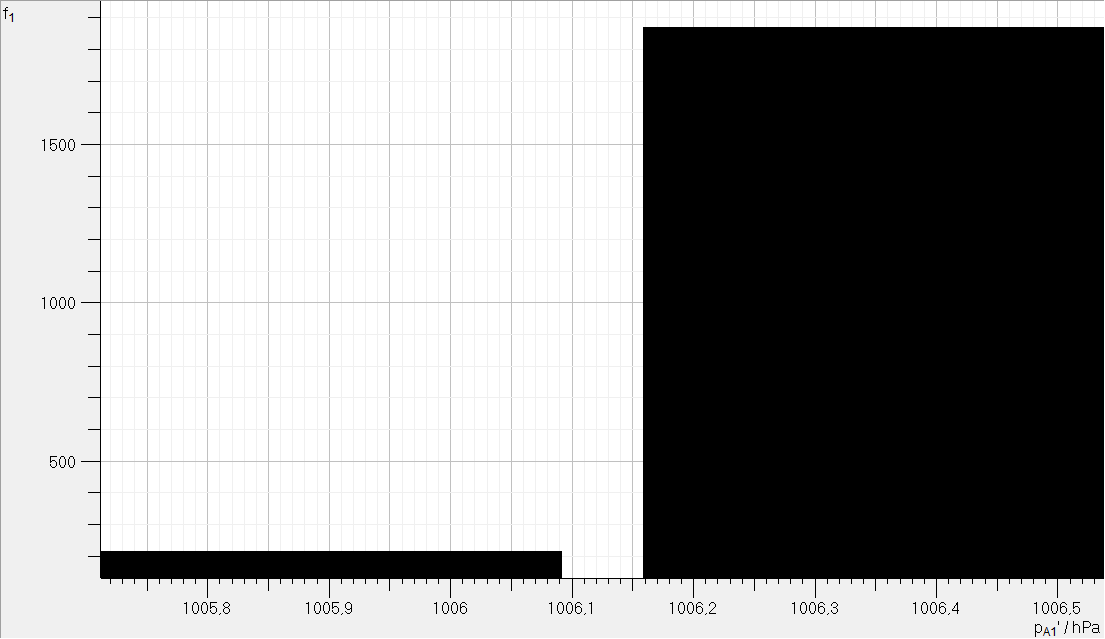
\includegraphics[width=0.49\textwidth]{Bilder/Zimmertemperatur_Druck_G2.png}}
\end{figure}

\begin{table}[H]\centering
\begin{tabular}{c|c|c}
 & Gruppe 1 & Gruppe 2 \\ 
\hline 
$P_M$ in hPa & 981.443 & 1006.265 \\ 
$\sigma_P$ in hPa & 0.370 & 0.348 \\  
\end{tabular} 
\end{table}
\end{frame}

\end{document}